%%% File encoding is ISO-8859-1 (also known as Latin-1)
%%% You can use special characters just like ä,ü and ñ
%%% LaTeX template by Manuel Kuehner, 2015

%%% If you use this template then please give credit like this:
%%% ----------------------------
% LaTeX code inspired by the LaTeX Thesis Template by Manuel Kuehner 
% www.bedienhaptik.de/latex-template/
%%% ----------------------------

% ##############################################
% Start: Template Preamble
% ##############################################
%

% Documentclass definition
\documentclass[11pt,a4paper,twoside, titlepage,headings = big, toc = bibliography,toc = listof]{scrbook}

% Loading additional packages from the KOMA-Script family
%%% File encoding is utf8
%%% You can use special characters just like ä,ü and ñ

% Special KOMA-Script package - I added it because I also use the float package in this template, see: 
% http://tex.stackexchange.com/questions/51867/koma-warning-about-toc
% CTAN: http://www.ctan.org/tex-archive/macros/latex/contrib/koma-script/doc
\usepackage{scrhack}

% Better support for marginnotes
% new command: \marginnote
% LaTeX standard command: \marginpar
% CTAN: http://www.ctan.org/pkg/marginnote
\usepackage{marginnote}

% Extended header and footer support
% CTAN: http://www.ctan.org/pkg/scrpage2
\usepackage[%
  	automark
  	,ilines
	,headsepline
	,footsepline
]{scrlayer-scrpage}

% Page layout definition
%%% File encoding is utf8
%%% You can use special characters just like ä,ü and ñ

% User friendly interface to change layout parameters
% CTAN: http://www.ctan.org/pkg/geometry
\usepackage{geometry}
\geometry{% siehe geometry.pdf (Figure 1)
	bottom=30mm,
	showframe=false, % For debugging: try true and see the layout frames
	margin=30mm,
	marginparsep=3mm,
	marginparwidth=20mm
}

% Standard packages
%%% File encoding is utf8
%%% You can use special characters just like ä,ü and ñ

\usepackage[utf8]{inputenc}

% Font Encoding is 'T1' -- important for special characters such as Umlaute ü or ä and special characters like ñ (enje)
% CTAN: http://www.ctan.org/pkg/fontenc
\usepackage[T1]{fontenc}

% Language support for 'english' (alternative 'ngerman' or 'french' for example)
% CTAN: http://www.ctan.org/pkg/babel
%\usepackage[english]{babel} 

% Package für Abkürzungsverzeichnis
\usepackage[printonlyused]{acronym}

% Package for smart diagrams
\usepackage{smartdiagram}

% Doing calculations with LaTeX units -- needed for the vertical line in the footer
% CTAN: http://www.ctan.org/pkg/calc
\usepackage{calc}

% Extended graphics support 
% There is also a package named 'graphics' - watch out!
% CTAN: http://www.ctan.org/pkg/graphicx
\usepackage{graphicx}

% Extendes support for floating objects (tables, figures), adds the [H] placing option (\begin{figure}[H]) which palces it "Here" (without any doubt).
% CTAN: http://www.ctan.org/pkg/float
\usepackage{float}


% Extendes support for special-text-floating of figures, which is not supported by package float.
%A word of warning: Wrapping figures in LaTeX will require a lot of manual adjustment of your document. There are several packages available for the task, but none of them works perfectly. Before you make the choice of including figures with text wrapping in your document, make sure you have considered all the options. For example, you could use a layout with two columns for your documents and have no text-wrapping at all.
%\usepackage{wrapfig}

\usepackage{pbox}

% Extended color support
% I use the command \definecolor for example. 
% Option 'Table': Load the colortbl package, in order to use the tools for coloring rows, columns, and cells within tables.
% CTAN: http://www.ctan.org/pkg/xcolor
\usepackage[table]{xcolor} 

% Nice tables
% CTAN: http://www.ctan.org/pkg/booktabs
\usepackage{booktabs}

% Better support for ragged left and right. Provides the commands \RaggedRight and \RaggedLeft. 
% Standard LaTeX commands are \raggedright and \raggedleft
% http://www.ctan.org/pkg/ragged2e
\usepackage{ragged2e}

% Create function plots directly in LaTeX
% CTAN: http://www.ctan.org/pkg/pgfplots
\usepackage{pgfplots}
\pgfplotsset{compat=1.11}

\usepackage{framed}

\usepackage{pdfpages}

% ####-Important-####
%
% Definition of the two main colors
% -----------------------
% The corresponding xcolor package ist loaded in the file 
% 01_Preamble/StandardPackages.tex
%
% ####-Important-####
\definecolor{mireviColorRed}{HTML}{fe0a1a}
\definecolor{mireviColorYellow}{HTML}{fe6000}
\definecolor{mireviColorOrange}{HTML}{ff8f00}
\definecolor{mireviColorGrey}{HTML}{3c3c3c}

% Customization of 
% - Floating Objects (Caption) 
% - Table of Contents (TOC)
% - List of Figures
% - List of Tables
% - Headings (like chapter, section, etc.)
%%% File encoding is utf8
%%% You can use special characters just like ä,ü and ñ

% ##############################################
% Start: Table of Contents (TOC) Customization
% ##############################################
%

% Level for numbered captions
\setcounter{secnumdepth}{5}

% Level of chapters that appear in Table of Contents
\setcounter{tocdepth}{5} % bis wohin ins Inhaltsverzeichnis aufnehmen
% -2 no caption at all
% -1 part
% 0  chapter
% 1  section    
% 2  subsection 
% 3  subsubsection
% 4  paragraph
% 5  subparagraph

% KOMA-Script code to adjust TOC
% Applying the color 'mireviColorOrange' which is defined in the main file (MainFile.tex)
\makeatletter
\addtokomafont{chapterentrypagenumber}{\color{mireviColorOrange}}
\addtokomafont{chapterentry}{\color{mireviColorOrange}}
\makeatother

%
% #######################
% End: Table of Contents (TOC) Customization
% #######################

% ##############################################
% Start: Floating Object Customization
% ##############################################
%

% Extended support for catioons of figures and tables etc.
% CTAN: http://www.ctan.org/pkg/caption
\usepackage[%
	font={small},
	labelfont={bf,sf},
	format=hang, % try plain or hang
	margin=5pt,
]{caption}
%

% #######################
% End: Floating Object Customization
% #######################

% ##############################################
% Start: Headings Customization
% ##############################################
%

% KOMA-Script code to customize the headings
% Applying the color 'mireviColorYellow' which is defined in the main file (MainFile.tex)
\addtokomafont{chapter}{\color{mireviColorYellow}}
\addtokomafont{section}{\color{mireviColorYellow}}
\addtokomafont{subsection}{\color{mireviColorYellow}}
\addtokomafont{subsubsection}{\color{mireviColorYellow}}
\addtokomafont{paragraph}{\color{mireviColorYellow}}
\addtokomafont{subparagraph}{\color{mireviColorYellow}}

% #######################
% End: Headings Customization
% #######################


% Customization of the header, footer and teh margin note
%%% File encoding is utf8
%%% You can use special characters just like ä,ü and ñ

% Custom command fpr the margin notes: \myMarginnote{Your Text}
% Comment on the \lineskiplimit=-\maxdimen:
% See http://tex.stackexchange.com/questions/49072/
% Without it the line spacing of the normal text was changed (ugly).
\newcommand{\myMarginnote}[1]{%
	\marginnote{% needs marginnote package
		\ifthispageodd{\RaggedRight}{\RaggedLeft}% needs ragged2e package
		\color{mireviColorOrange}%
		\lineskiplimit=-\maxdimen% 
		\normalfont\sffamily\scriptsize%
		#1}%
}

% ##############################################
% Start: Header and Footer Customization
% ##############################################
%

% KOMA-Script code for header and footer font
\setkomafont{pageheadfoot}{%
	\normalfont\sffamily\bfseries
	}
\setkomafont{pagefoot}{%
	\normalfont\sffamily
	}
\setkomafont{pagenumber}{%
	\normalfont\rmfamily
	}

% Define width of header
\setheadwidth[0pt]{textwithmarginpar}

% Define with of header line
%\setheadsepline{0.4pt}

% Define width of footer
\setfootwidth[0pt]{text}
% Define with of footer line (here: no line)
%\setfootsepline[text]{0pt}

% setheadsepline{0.4pt} und setfootsepline[text]{0pt} erstetzt duruch:
\KOMAoptions{footsepline=0pt}
\KOMAoptions{headsepline=0.4pt}
% Dann gabs keine Warnings mehr (vom unwissenden Mitja gehackt!)




% Some calculations
% calc package is needed which is loaded here: 01_Preamble/CommonPackages.tex
% If you want to understand the calculations visit:
% http://en.wikibooks.org/wiki/LaTeX/Page_Layout
\newlength{\myLenghthFootAbstand}
\setlength{\myLenghthFootAbstand}{\paperheight-1in-\topmargin- \headheight-\headsep-\textheight-\footskip}
\newlength{\myLenghthTemp}
\setlength{\myLenghthTemp}{\myLenghthFootAbstand+\baselineskip}

% Define content of header and footer
% Using some scrpage2 commands here. The scrpage2 package is loaded here: 01_Preamble/KOMA-Script-Packages.tex
% Some LaTeX magic...
% Clear all defaults
\clearscrheadfoot
% Header
\ohead{%
	\textcolor{mireviColorOrange}{\headmark}
	}
% Left (even page numbers) footer
\lefoot%
[% scrplain style (begin)
	\setlength{\unitlength}{\myLenghthFootAbstand}%
	\begin{picture}(0,0)%
		\put(0,-1)%
		{%
			\makebox(0,0)[lb]%
			{%
				\rule{0.4pt}{\myLenghthTemp}%
			}%
		}%
	\end{picture}\llap{\pagemark~}%
]% scrplain style (end)
%
{% scrheadings style (begin)
	\setlength{\unitlength}{\myLenghthFootAbstand}%
	\begin{picture}(0,0)%
		\put(0,-1)%
		{%
			\makebox(0,0)[lb]%
			{%
				\rule{0.4pt}{\myLenghthTemp}%
			}%
		}%
	\end{picture}\llap{\pagemark~}%
}% scrheadings style (end)

% Right (odd page numbers) footer
\rofoot%
[% scrplain style (begin)
	\rlap{~\pagemark}%%
	\setlength{\unitlength}{\myLenghthFootAbstand}%
	\begin{picture}(0,0)%
		\put(0,-1)%
		{%
			\makebox(0,0)[lb]%
			{%
				\rule{0.4pt}{\myLenghthTemp}%
			}%
		}%
	\end{picture}%
]% scrplain style (end)
%
{% scrplain style (begin)
	\rlap{~\pagemark}%%
	\setlength{\unitlength}{\myLenghthFootAbstand}%
	\begin{picture}(0,0)%
		\put(0,-1)%
		{%
			\makebox(0,0)[lb]%
			{%
				\rule{0.4pt}{\myLenghthTemp}%
			}%
		}%
	\end{picture}%
}% scrplain style (end)

%
% #######################
% End: Header and Footer Customization
% #######################

% Optimize paragraphs (avoid overfull... warnings)
%%% File encoding is utf8
%%% You can use special characters just like ä,ü and ñ

% This is an suggestion from Axel Reichert (LaTeX package author)
% See CTAN: http://www.ctan.org/author/reichert
% See CTAN: http://www.ctan.org/pkg/l2tabu-english (Cgapter: 1.8 Should I use \sloppy?)

\tolerance 1414
\hbadness 1414
\emergencystretch 1.5em
\hfuzz 0.3pt
\widowpenalty=10000
\vfuzz \hfuzz
\raggedbottom

% PDF related packages
%%% File encoding is utf8
%%% You can use special characters just like ä,ü and ñ

% Package for PDF features such as bookmarks and hyperlinks. 
% Important: Should be loaded at the end.
% CTAN: http://www.ctan.org/pkg/hyperref
\usepackage[%
pdftitle={Hier Titel der Arbeit},%
pdfauthor={Hier Name des Studenten},%
pdfcreator={LaTeX},
pdfsubject={Hier Art der Arbeit},
pdfkeywords={passende keywords},
bookmarks, % Create bookmarks
bookmarksopen=true, % Unfold bookmatk tree in PDF viewer when document is opened
bookmarksopenlevel=1, % Level of unfolding
bookmarksnumbered=true, % Number bookmarks
hidelinks, % do not highlight hyperlinks -- looks ugly
% Ansicht beim Öffnen
pdfpagelabels=true, % See manual...
plainpages=false, % See manual...
hyperfootnotes=true, % Hyperlinks for footnotes
hyperindex=true, % Indexeinträage verweisen auf Text
]{hyperref}

% PDF related packages
%%% File encoding is utf8
%%% You can use special characters just like ä,ü and ñ

% Package to create test text -- just for demonstration purposes
% The command \blindtext produces a test text -- good for testing the layout
% CTAN: http://www.ctan.org/pkg/blindtext
\usepackage[]{blindtext}
% The custom command \myMarginnote is defined in the file: 
% 01_Preamble/HeaderFooterMarginnote.tex
\renewcommand{\blindmarkup}[1]{\myMarginnote{#1}}

%
% #######################
% Ende: Template Preamble
% #######################

% ##############################################
% Start: Document
% ##############################################
%
% ------------------------------------------------------------------
\begin{document}
\frontmatter
% Title page
%%% File encoding is utf8
%%% You can use special characters just like ä,ü and ñ

\begin{titlepage}
\begin{center}
	\vspace*{1.7cm}	
	\huge Hier Titel einfügen \\
	\vspace*{1.0cm}
	\Large Bachelorthesis / Masterthesis (eng.: Bachelor's / Master's Thesis)\\B.Sc. / B.Eng. / M.Sc. Studiengang\\Name Autor\\
	
	\vspace{4.0cm}
	
	\begin{figure}[htb]
		\begin{center}
			
\includegraphics[width=0.75\textwidth]{03_GraphicFiles/title_Logos.png}
		\end{center}
	\end{figure}
	\vspace{0.9cm}
	\Large Supervision: \\ 
	\Large Name 1. Prüfer \\
%	\vspace{0.2cm}
	\Large Name 2. Prüfer
	
	\vspace{1.5cm}
	\Large D\"usseldorf\\
	\Large Monat Jahr\\
\end{center}
\end{titlepage}
% Empty page after title page
\cleardoublepage

% Activate header and footer defined in the file:
% 01_Preamble/HeaderFooterMarginnote.tex
\pagestyle{scrheadings}

% Activate roman numbering (e. g. xii)	
\pagenumbering{roman}
% Start with page 1 (I)
\setcounter{page}{1}
% Prologue
%%% File encoding is utf8
%%% You can use special characters just like ä,ü and ñ

% Chapter without numbering but with appearance in the Table of Contents
% \addchap is a command from KOMA-Script
%\addchap{Prologue}
%
%\Blindtext[3][1]
\addchap{Statutory Declaration}

\normalsize
I declare that I have authored this thesis independently, that I have not used other than the declared
sources / resources, and that I have explicitly marked all material which has been quoted either
literally or by content from the used sources.
\vspace*{3.0cm}

\begin{table}[H]
	\centering
	\begin{tabular}{ c c}
		.......................\hspace*{5.0cm}  & ............................................ \\
		date \hspace*{5.1cm} & signature \\
	\end{tabular}
\end{table}



%%% File encoding is utf8
%%% You can use special characters just like ä,ü and ñ

% Chapter without numbering but with appearance in the Table of Contents
% \addchap is a command from KOMA-Script
%\addchap{Prologue}
%
%\Blindtext[3][1]
\addchap{}
\emph{Hier vielleicht eine nette Danksagung}

%Icons of Menus are made by Freepik from www.flaticon.com is licensed by CC 3.0 --> Keine Icons mehr von drin

%Thanks to Lava Labs, Christian Laskawi, Timo, Sebastian, Mitja, Basti Dewitz, etc.




% Abstract
%%% File encoding is utf8
%%% You can use special characters just like ä,ü and ñ

% Chapter without numbering but with appearance in the Table of Contents
% \addchap is a command from KOMA-Script
\addchap{Abstract}
Zusammenfassung (ca. 200 Wörter - Englisch)


\textcolor{mireviColorOrange}{\textbf{Keywords:}} Hier passende Keywords (Englisch)


\addchap{Zusammenfassung}
Zusammenfassung (ca. 200 Wörter - Deutsch)


Die Zusammenfassung dient dem Leser dazu, sich einen ersten Überblick über die Arbeit zu verschaffen. Dazu sollten in der Zusammenfassung die Aufgabenstellung, die erarbeiteten Lösungskonzepte, der Nutzen und ein kurzes Fazit aufgeführt sein. Eine Thesis muss \textbf{immer eine englische und deutsche Zusammenfassung} beinhalten. Die Sprache der Thesis ist wählbar und kann auf deutsch und auf englisch geschrieben werden. Andere Sprachen sind nicht zugelassen. 

\textcolor{mireviColorOrange}{\textbf{Keywords:}} Hier passende Keywords (Deutsch)

% Table of Contents and Lost of Figures/Tables
%%% File encoding is utf8
%%% You can use special characters just like ä,ü and ñ

% Table of Contents (TOC)
% Special code so that it appears as a bookmark in the PDF viewer
\phantomsection
\pdfbookmark[0]{Table of Contents}{toc} % <-- Please edit the name if you want a different text as a bookbarl for the Table of Contents
\tableofcontents
% List of Figures
\listoffigures
% List of Tables
\listoftables
\input{02_Chapters/Abkürzungsverzeichnis}

% Introduction


%%% File encoding is utf8
%%% You can use special characters just like ä,ü and ñ
\mainmatter
\chapter{Einleitung}
In der Einleitung einer Abschlussarbeit sollte die Thematik der Arbeit und die Motivation, wieso dieses Thema bearbeitet wird, beschrieben und begründet werden. Der Leser soll eine Vorstellung von dem Inhalt der Arbeit bekommen. Optional können die einzelnen Kapitel der Arbeit kurz vorgestellt und beschrieben werden. Die Problemstellung und der Forschungsstand können in eigenen Unterkapiteln beschrieben werden.
Wichtig: Entweder es gibt mind. 2 Unterkapitel oder kein Unterkapitel! Gibt es nur einen Unterpunkt sollte dieser unbedingt in das Überkapitel mit einbezogen und auf den Unterpunkt verzichtet werden!

\section{Motivation/Problemstellung}
Lorem ipsum dolor sit amet, consetetur sadipscing elitr, sed diam nonumy eirmod tempor invidunt ut labore et dolore magna aliquyam erat, sed diam voluptua. At vero eos et accusam et justo duo dolores et ea rebum. Stet clita kasd gubergren, no sea takimata sanctus est Lorem ipsum dolor sit amet. Lorem ipsum dolor sit amet, consetetur sadipscing elitr, sed diam nonumy eirmod tempor invidunt ut labore et dolore magna aliquyam erat, sed diam voluptua. At vero eos et accusam et justo duo dolores et ea rebum. Stet clita kasd gubergren, no sea takimata sanctus est Lorem ipsum dolor sit amet. 

\section{Zielsetzung}
Lorem ipsum dolor sit amet, consetetur sadipscing elitr, sed diam nonumy eirmod tempor invidunt ut labore et dolore magna aliquyam erat, sed diam voluptua. At vero eos et accusam et justo duo dolores et ea rebum. Stet clita kasd gubergren, no sea takimata sanctus est Lorem ipsum dolor sit amet. Lorem ipsum dolor sit amet, consetetur sadipscing elitr, sed diam nonumy eirmod tempor invidunt ut labore et dolore magna aliquyam erat, sed diam voluptua. At vero eos et accusam et justo duo dolores et ea rebum. Stet clita kasd gubergren, no sea takimata sanctus est Lorem ipsum dolor sit amet.



% Activate arabic numbering (e. g. 12)	

%%% File encoding is utf8
%%% You can use special characters just like ä,ü and ñ

\chapter{Kapitel 2}\label{cha:rr}
Lorem ipsum dolor sit amet, consetetur sadipscing elitr, sed diam nonumy eirmod tempor invidunt ut labore et dolore magna aliquyam erat, sed diam voluptua. At vero eos et accusam et justo duo dolores et ea rebum. Stet clita kasd gubergren, no sea takimata sanctus est Lorem ipsum dolor sit amet. Lorem ipsum dolor sit amet, consetetur sadipscing elitr, sed diam nonumy eirmod tempor invidunt ut labore et dolore magna aliquyam erat, sed diam voluptua. At vero eos et accusam et justo duo dolores et ea rebum. Stet clita kasd gubergren, no sea takimata sanctus est Lorem ipsum dolor sit amet.

\section{Unterkapitel 2.1}\label{cha:unterkapitel}
Lorem ipsum dolor sit amet, consetetur sadipscing elitr, sed diam nonumy eirmod tempor invidunt ut labore et dolore magna aliquyam erat, sed diam voluptua. At vero eos et accusam et justo duo dolores et ea rebum. Stet clita kasd gubergren, no sea takimata sanctus est Lorem ipsum dolor sit amet. Lorem ipsum dolor sit amet, consetetur sadipscing elitr, sed diam nonumy eirmod tempor invidunt ut labore et dolore magna aliquyam erat, sed diam voluptua. At vero eos et accusam et justo duo dolores et ea rebum. Stet clita kasd gubergren, no sea takimata sanctus est Lorem ipsum dolor sit amet.

Hier ein Beispiel für eine \textbf{unnumerierte} Liste:

\begin{itemize}
	\item Punkt
	\item Punkt
	\item Punkt
	\item Punkt
\end{itemize}

\section{Unterkapitel 2.2}
Lorem ipsum dolor sit amet, consetetur sadipscing elitr, sed diam nonumy eirmod tempor invidunt ut labore et dolore magna aliquyam erat, sed diam voluptua. At vero eos et accusam et justo duo dolores et ea rebum. Stet clita kasd gubergren, no sea takimata sanctus est Lorem ipsum dolor sit amet. Lorem ipsum dolor sit amet, consetetur sadipscing elitr, sed diam nonumy eirmod tempor invidunt ut labore et dolore magna aliquyam erat, sed diam voluptua. At vero eos et accusam et justo duo dolores et ea rebum. Stet clita kasd gubergren, no sea takimata sanctus est Lorem ipsum dolor sit amet.

\subsection{Unterunterkapitel 2.2.1}
Lorem ipsum dolor sit amet, consetetur sadipscing elitr, sed diam nonumy eirmod tempor invidunt ut labore et dolore magna aliquyam erat, sed diam voluptua. At vero eos et accusam et justo duo dolores et ea rebum. Stet clita kasd gubergren, no sea takimata sanctus est Lorem ipsum dolor sit amet. Lorem ipsum dolor sit amet, consetetur sadipscing elitr, sed diam nonumy eirmod tempor invidunt ut labore et dolore magna aliquyam erat, sed diam voluptua. At vero eos et accusam et justo duo dolores et ea rebum. Stet clita kasd gubergren, no sea takimata sanctus est Lorem ipsum dolor sit amet.

Hier ein Beispiel für eine \textbf{nummerierte} Liste mit hervorgehobener Schrift:
%\newpage
\begin{enumerate}
	\item \textbf{Punkt}
	\item \textbf{Punkt}
	\item \textbf{Punkt}
\end{enumerate}

\subsection{Unterunterkapitel 2.2.2}
Lorem ipsum dolor sit amet, consetetur sadipscing elitr, sed diam nonumy eirmod tempor invidunt ut labore et dolore magna aliquyam erat, sed diam voluptua. At vero eos et accusam et justo duo dolores et ea rebum. Stet clita kasd gubergren, no sea takimata sanctus est Lorem ipsum dolor sit amet. Lorem ipsum dolor sit amet, consetetur sadipscing elitr, sed diam nonumy eirmod tempor invidunt ut labore et dolore magna aliquyam erat, sed diam voluptua. At vero eos et accusam et justo duo dolores et ea rebum. Stet clita kasd gubergren, no sea takimata sanctus est Lorem ipsum dolor sit amet.

%%% File encoding is utf8
%%% You can use special characters just like ä,ü and ñ

\chapter{Formatierung und Umgang mit der Vorlage}
In diesem Kapitel wird die Handhabung mit dem Template vorgestellt und anhand verschiedener Beispiele gezeigt. Die Struktur des Dokuments soll simpel gehalten werden und basiert auf einer einfachen Ordnerstruktur. Diese ist wichtig, um auf die verschiedenen Dateien über das MainFile zugreifen zu können. Daher sollte die Ordnerstruktur unbedingt beibehalten werden.

\section{Preambles}
Die Preambles definieren die Formatierung (Schriftgröße, Seitenzahlen, Farben, etc.) des Dokuments und sollten \textbf{nicht} bearbeitet werden! Nur die Datei \textbf{PDF-Related} kann bearbeitet und die entsprechenden "Felder" ausgefüllt werden.

\section{Kapitel}
Jedes Oberkapitel hat seine eigene .tex Datei. Diese Dateien liegen in dem Ordner für Kapitel. Möchte man ein neues Kapitel erstellen, so legt man einfach eine neue Datei an und legt sie in diesem Ordner ab. Das Kapitel muss dann über das MainFile (siehe \ref{cha:mainFile}) in das Dokument eingebunden werden. Verschiedene Kapitel lassen sich auch, ähnlich zu einem Wiki-Artikel, untereinander verlinken. Dazu vergibt man dem jeweiligen Kapitel ein Label und ein Kürzel, über welches das jeweilige Kapitel angesprochen werden kann.

\section{MainFile}\label{cha:mainFile}
Im MainFile werden die verschiedenen Kapitel zu einem Dokument zusammengefügt. Hier werden keine Texte geschrieben, sondern nur die Dateien aus den entsprechenden Ordnern aufgerufen (\emph{siehe Abbildung}). Bearbeitet wird das MainFile erst ab dem Tag \textbf{begin document}. Die input-Befehle binden die Preambles in das Dokument ein.

\begin{figure}[H]
    \centering
    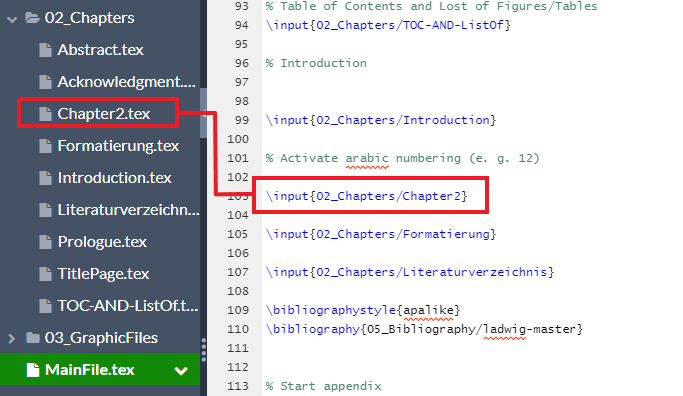
\includegraphics[width=\textwidth]{03_GraphicFiles/MainFile.png}
    \caption{Code-Snippet MainFile (Overleaf)}
    \label{fig:mainFile}
\end{figure}

\section{Abbildungen und Tabellen}
In diesem Abschnitt wird gezeigt, wie Abbildungen und Tabellen in das Dokument eingebunden werden. Das Abbildungs- und Tabellenverzeichnis wird automatisch aktualisiert sobald man eine Abbildung oder Tabelle korrekt einbindet und die PDF-Datei kompiliert.

\subsection{Abbildungen} \label{cha:figures}
Für Abbildungen wird ebenfalls ein eigener Ordner angelegt, über den die Dateien aufgerufen werden können.

\begin{figure}[H]
    \centering
    \includegraphics[width=\textwidth]{03_GraphicFiles/BilderEinfügen.png}
    \caption{Abbildungen korrekt einfügen}
    \label{fig:picture}
\end{figure}

Das \textbf{[H]}, in der Abbildung gelb markiert, sorgt dafür, dass das jeweilige Bild genau an der Stelle im Dokument eingefügt wird, an der sich das Bild auch im Code befindet. Ansonsten kann es passieren, dass die Bilder nicht an der richtigen Stelle im Dokument, eventuell sogar in einem anderen Kapitel, abgebildet werden.

\newpage
\subsection{Tabellen und Diagramme}
Tabellen lassen sich einfach erstellen, auch das Layout der Tabellen lässt sich schnell ändern.

\begin{table}[H]
	\centering
	\begin{tabular}{|| c | c | c | c | c | c ||}
	    \hline
		Spalte & Spalte & Spalte & Spalte & Spalte & Spalte \\ [0.5ex]
		\hline\hline
		Inhalt & Inhalt & Inhalt & Inhalt & Inhalt & Inhalt \\
		Zeile & Zeile & Zeile & Zeile & Zeile & Zeile \\
		Inhalt & Inhalt & Inhalt & Inhalt & Inhalt & Inhalt \\
		Zeile & Zeile & Zeile & Zeile & Zeile & Zeile \\
		\hline
	\end{tabular}
	\caption{Eine Tabelle erstellen}
	\label{tab:newTable}
\end{table}

\begin{figure}[H]
    \centering
    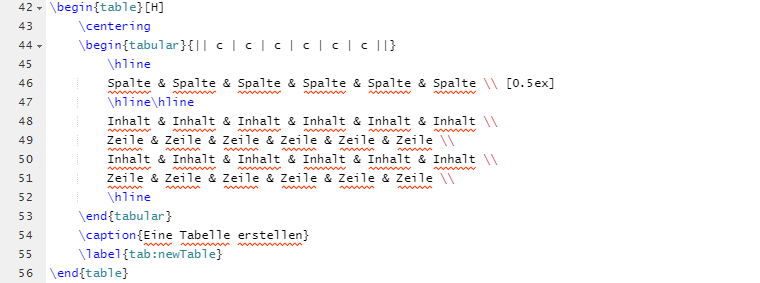
\includegraphics[width=\textwidth]{03_GraphicFiles/TabellenErstellen.PNG}
    \caption{Code-Snippet für Tabellen}
    \label{fig:createTable}
\end{figure}

Es lassen sich auch vorgefertigte Diagramme über LaTex erstellen und verändern. Verschiedene Arten von Diagrammen können mit dem \emph{smartdiagram-package} einfach und schnell generiert werden. Das Package stellt verschiedene Arten von Diagrammen bereit. Möchte man diese nutzen, so sollte man sich auf der entsprechenden Internetseite informieren. 

Hier zwei Beispiel-Diagramme:
\begin{figure}[H]
    \centering
    \smartdiagram[flow diagram:horizontal]{Schritt 1, Schritt 2, Schritt 3, Schritt 4, Schritt 5}
    \caption{Ein Flussdiagramm mit schönen Farben}
    \label{fig:flowdiagram}
\end{figure}

Die Diagramme werden erstellt wie Abbildungen (siehe \ref{cha:figures}). Anstatt \emph{includegraphics} wird bei Diagrammen einfach \emph{smartdiagram} aufgerufen. In den eckigen Klammern wird dann die Art des Diagramms definiert und in den geschweiften Klammern der Inhalt (siehe \ref{fig:diagrams}). Die Diagramme werden so auch im Abbildungsverzeichnis gelistet und können mit einer passenden Beschreibung versehen werden.

\begin{figure}
    \centering
    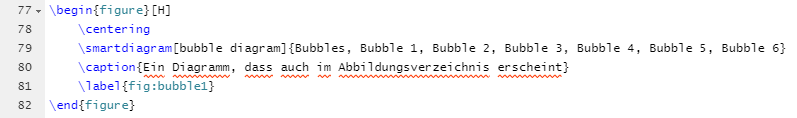
\includegraphics[width=\textwidth]{03_GraphicFiles/smartdiagram.PNG}
    \caption{How to diagram}
    \label{fig:diagrams}
\end{figure}

\begin{figure}[H]
    \centering
    \smartdiagram[bubble diagram]{Bubbles, Bubble 1, Bubble 2, Bubble 3, Bubble 4, Bubble 5, Bubble 6}
    \caption{Ein Diagramm, welches auch im Abbildungsverzeichnis gelistet wird}
    \label{fig:bubble1}
\end{figure}

\section{Literaturverzeichnis}
Für das Literaturverzeichnis ist es empfehlenswert ein Programm, beispielsweise Citavi, zu nutzen. Es gibt einige Programme, die sich problemlos in Verbindung mit LaTex nutzen lassen können. Über Citavi, beispielsweise, lässt sich direkt eine BibTex-Datei erstellen, die sich einfach in das Dokument einbinden lässt. \emph{Beispiel-Literatur für Literaturverzeichnis -} \cite{Butterworth1992}.
\emph{Beispiel-Literatur für Literaturverzeichnis -} \cite{Clark1976}
Für den Umgang mit Litertaturmanagement-Programmen und LaTex gibt es zahlreiche Tutorials, beispielsweise für  \href{https://www.youtube.com/watch?v=GmyCcvXrSDI}{Umgang mit LaTex und Citavi}






\bibliographystyle{apalike}
\bibliography{05_Bibliography/Literaturverzeichnis}


% Start appendix
\appendix

%Appendix A
%%% File encoding is utf8
%%% You can use special characters just like ä,ü and ñ
%\addchap{Appendix}
\chapter{Appendix}\label{cha: appendixA}
Im Anhang werden alle Bilder, Dateien und Code-Snippets dargestellt, die wichtig für das Verständnis und Reproduzierbarkeit sind, jedoch zu viel Platz im Hauptteil der Arbeit einnehmen würden. Fragebögen, Daten aus Evaluationen, eventuell Fragebögen und andere Informationen können hier bereitgestellt werden. Der Anhang verfügt über ein Label und kann dadurch in anderen Kapiteln referenziert werden.

\section{Bilder von Sachen}
\begin{figure}[H]
	\centering  
	\includegraphics[width=\textwidth]{03_GraphicFiles/BilderEinfügen.png}
	\caption{Hier passende Caption einfügen}
	\label{fig:picture01}
\end{figure}

\begin{figure}[H]
	\centering  
	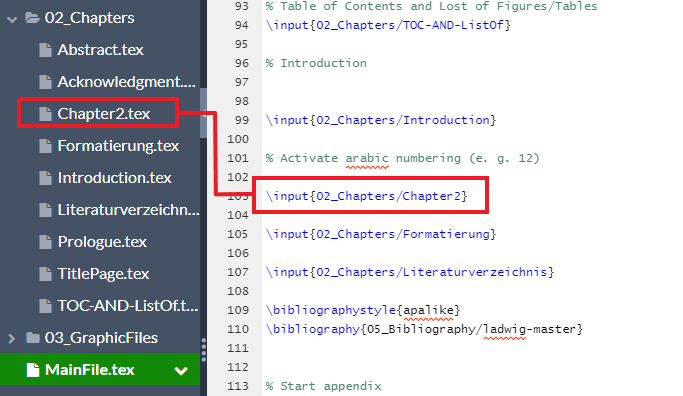
\includegraphics[width=\textwidth]{03_GraphicFiles/MainFile.png}
	\caption{Hier passende Caption einfügen}
	\label{fig:picture02}
\end{figure}

\begin{figure}[H]
	\centering  
	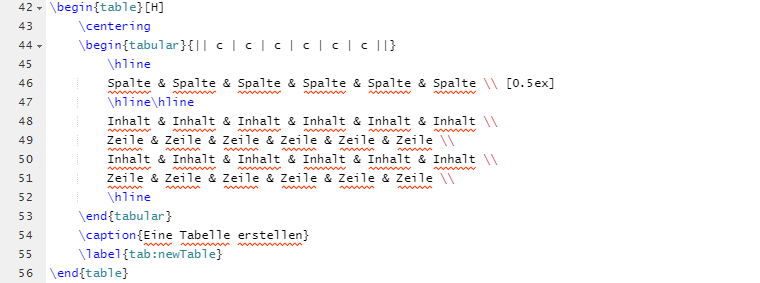
\includegraphics[width=\textwidth]{03_GraphicFiles/TabellenErstellen.PNG}
	\caption{Hier passende Caption einfügen}
	\label{fig:picture03}
\end{figure}

\newpage
\section{PDFs verlinken}\label{cha:pdfLink}
Es können auch bestimmte Seiten aus PDF-Dateien im Anhang dargestellt werden. Dazu muss man, wie bei Abbildungen, die gewünschte PDF in den passenden Ordner ablegen. Auf der folgenden Seite findet sich ein Ausschnitt aus dem Leitfaden für Masterarbeiten bei MIREVI.

\includepdf[pages={5}]{99_AppendixFiles/Leitfaden Abschlussarbeit.pdf}


% Appendix B
%\input{02_Chapters/AppendixExampleChapterB.tex}

\end{document}
% ------------------------------------------------------------------
%
% #######################
% End: Document
% #######################
